
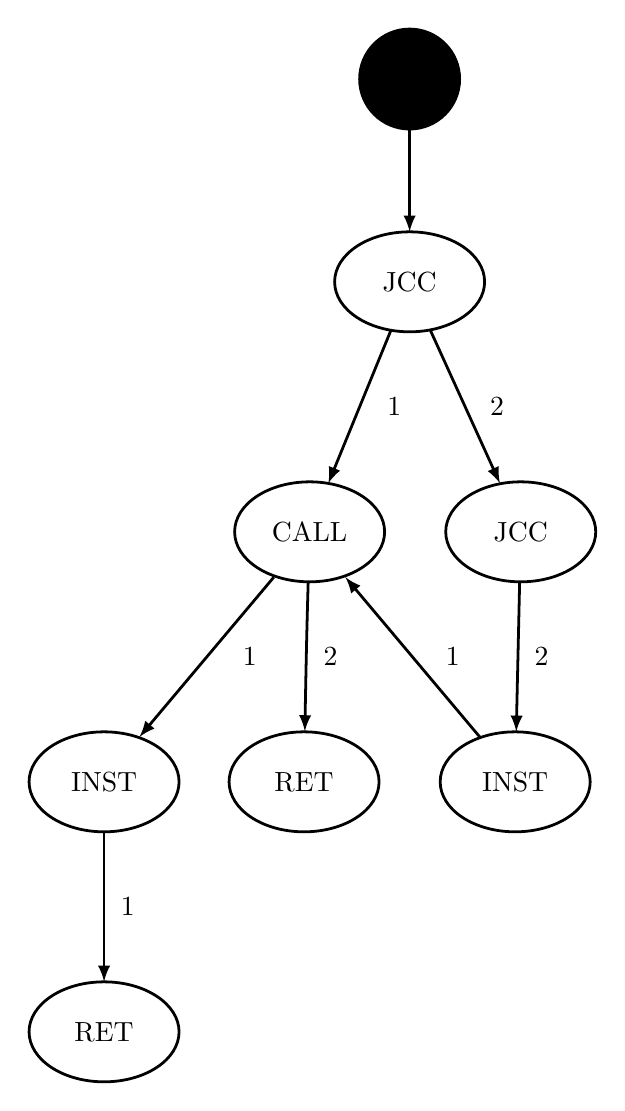
\begin{tikzpicture}[>=latex,line join=bevel,]
  \pgfsetlinewidth{1bp}
%%
\begin{scope}
  \pgfsetstrokecolor{black}
  \definecolor{strokecol}{rgb}{1.0,1.0,1.0};
  \pgfsetstrokecolor{strokecol}
  \definecolor{fillcol}{rgb}{1.0,1.0,1.0};
  \pgfsetfillcolor{fillcol}
  \filldraw (0.0bp,0.0bp) -- (0.0bp,379.0bp) -- (204.0bp,379.0bp) -- (204.0bp,0.0bp) -- cycle;
\end{scope}
\begin{scope}
  \pgfsetstrokecolor{black}
  \definecolor{strokecol}{rgb}{1.0,1.0,1.0};
  \pgfsetstrokecolor{strokecol}
  \definecolor{fillcol}{rgb}{1.0,1.0,1.0};
  \pgfsetfillcolor{fillcol}
  \filldraw (0.0bp,0.0bp) -- (0.0bp,379.0bp) -- (204.0bp,379.0bp) -- (204.0bp,0.0bp) -- cycle;
\end{scope}
  \pgfsetcolor{black}
  % Edge: 3 -> 6
  \draw [->] (176.6bp,179.61bp) .. controls (176.32bp,167.24bp) and (175.94bp,150.37bp)  .. (175.39bp,126.05bp);
  \definecolor{strokecol}{rgb}{0.0,0.0,0.0};
  \pgfsetstrokecolor{strokecol}
  \draw (184.5bp,153.0bp) node {2};
  % Edge: 6 -> 2
  \draw [->] (162.26bp,124.15bp) .. controls (150.74bp,137.85bp) and (133.61bp,158.22bp)  .. (113.89bp,181.67bp);
  \draw (152.5bp,153.0bp) node {1};
  % Edge: 4 -> 7
  \draw [->] (27.0bp,89.614bp) .. controls (27.0bp,77.24bp) and (27.0bp,60.369bp)  .. (27.0bp,36.05bp);
  \draw (35.5bp,63.0bp) node {1};
  % Edge: 1 -> 3
  \draw [->] (144.52bp,270.45bp) .. controls (150.39bp,257.54bp) and (158.64bp,239.39bp)  .. (169.51bp,215.48bp);
  \draw (168.5bp,243.0bp) node {2};
  % Edge: 0 -> 1
  \draw [->] (137.0bp,342.81bp) .. controls (137.0bp,334.79bp) and (137.0bp,325.05bp)  .. (137.0bp,306.03bp);
  % Edge: 2 -> 5
  \draw [->] (100.48bp,179.91bp) .. controls (100.31bp,174.21bp) and (100.14bp,167.83bp)  .. (100.0bp,162.0bp) .. controls (99.803bp,153.68bp) and (99.62bp,144.63bp)  .. (99.282bp,126.19bp);
  \draw (108.5bp,153.0bp) node {2};
  % Edge: 1 -> 2
  \draw [->] (130.23bp,270.45bp) .. controls (125.0bp,257.66bp) and (117.66bp,239.74bp)  .. (107.74bp,215.48bp);
  \draw (131.5bp,243.0bp) node {1};
  % Edge: 2 -> 4
  \draw [->] (88.11bp,181.67bp) .. controls (76.544bp,167.92bp) and (59.411bp,147.54bp)  .. (39.742bp,124.15bp);
  \draw (79.5bp,153.0bp) node {1};
  % Node: 1
\begin{scope}
  \definecolor{strokecol}{rgb}{0.0,0.0,0.0};
  \pgfsetstrokecolor{strokecol}
  \draw (137.0bp,288.0bp) ellipse (27.0bp and 18.0bp);
  \draw (137.0bp,288.0bp) node {JCC};
\end{scope}
  % Node: 0
\begin{scope}
  \definecolor{strokecol}{rgb}{0.0,0.0,0.0};
  \pgfsetstrokecolor{strokecol}
  \definecolor{fillcol}{rgb}{0.0,0.0,0.0};
  \pgfsetfillcolor{fillcol}
  \filldraw [opacity=1] (137.0bp,361.0bp) ellipse (18.0bp and 18.0bp);
\end{scope}
  % Node: 3
\begin{scope}
  \definecolor{strokecol}{rgb}{0.0,0.0,0.0};
  \pgfsetstrokecolor{strokecol}
  \draw (177.0bp,198.0bp) ellipse (27.0bp and 18.0bp);
  \draw (177.0bp,198.0bp) node {JCC};
\end{scope}
  % Node: 2
\begin{scope}
  \definecolor{strokecol}{rgb}{0.0,0.0,0.0};
  \pgfsetstrokecolor{strokecol}
  \draw (101.0bp,198.0bp) ellipse (27.0bp and 18.0bp);
  \draw (101.0bp,198.0bp) node {CALL};
\end{scope}
  % Node: 5
\begin{scope}
  \definecolor{strokecol}{rgb}{0.0,0.0,0.0};
  \pgfsetstrokecolor{strokecol}
  \draw (99.0bp,108.0bp) ellipse (27.0bp and 18.0bp);
  \draw (99.0bp,108.0bp) node {RET};
\end{scope}
  % Node: 4
\begin{scope}
  \definecolor{strokecol}{rgb}{0.0,0.0,0.0};
  \pgfsetstrokecolor{strokecol}
  \draw (27.0bp,108.0bp) ellipse (27.0bp and 18.0bp);
  \draw (27.0bp,108.0bp) node {INST};
\end{scope}
  % Node: 7
\begin{scope}
  \definecolor{strokecol}{rgb}{0.0,0.0,0.0};
  \pgfsetstrokecolor{strokecol}
  \draw (27.0bp,18.0bp) ellipse (27.0bp and 18.0bp);
  \draw (27.0bp,18.0bp) node {RET};
\end{scope}
  % Node: 6
\begin{scope}
  \definecolor{strokecol}{rgb}{0.0,0.0,0.0};
  \pgfsetstrokecolor{strokecol}
  \draw (175.0bp,108.0bp) ellipse (27.0bp and 18.0bp);
  \draw (175.0bp,108.0bp) node {INST};
\end{scope}
%
\end{tikzpicture}

